\documentclass{beamer}


\usepackage[utf8]{inputenc}
\usepackage[T1]{fontenc}
\usepackage[spanish]{babel}
\usepackage[normalem]{ulem}
\usepackage{longtable}
\usepackage{hhline}

\usepackage{natbib}
%sort,comma
\usepackage{lmodern}
\usepackage{stmaryrd}
\usepackage{marginnote}
\resetcounteronoverlays{exx} %Esto es para que el comando \pause no reinicie el conteo de los ejemplos 
\usepackage{expex}
\usepackage{qtree, tree-dvips, graphicx, caption}
\usepackage{hyperref}
\usepackage{tikz}
\usepackage{xurl}
%\usepackage{tikz-qtree}

\usetheme{CambridgeUS} %Tema.
\setbeamercolor{block body}{fg=grey,bg=yellow!05} % Con esto se manejan los colores de los bloques. Con fg se maneja el color de la letra, con bg el color de fondo.
\usepackage{verbatim}
\usepackage{xcolor}
\usepackage{listings}
\lstset{
    language=[LaTeX]TeX,
    breaklines=true,
    basicstyle=\tt\scriptsize,
    keywordstyle=\color{blue},
    identifierstyle=\color{magenta}}

\usepackage{gb4e}

\title{Expresiones regulares}
\date{Miércoles 20/03/2024}
\author[Fernando Carranza]{Fernando Carranza\\fernandocarranza86@gmail.com}

\begin{document}



\begin{frame}
\maketitle
\end{frame}

\begin{comment}

\section{ChatGPT}
\begin{frame}
¿Qué opina ChatGPT sobre las expresiones regulares y su utilidad en lingüística?
\end{frame}

\begin{frame}{Expresiones regulares según ChatGPT}
Las expresiones regulares son secuencias de caracteres que conforman un patrón de búsqueda, utilizadas para encontrar cadenas de texto que coincidan con ese patrón. Estos patrones se definen mediante una sintaxis específica que permite buscar y manipular texto de manera eficiente.

Para los lingüistas, las expresiones regulares pueden ser herramientas muy útiles en varios aspectos:

\end{frame}

\begin{frame}[allowframebreaks]{Expresiones regulares según ChatGPT}
\begin{enumerate}
\item \textbf{Análisis lingüístico}: Permiten buscar patrones específicos en textos, lo que puede ayudar en tareas de análisis lingüístico como la identificación de estructuras gramaticales, la extracción de información semántica o el reconocimiento de patrones fonéticos.

\item \textbf{Normalización de texto}: En la lingüística computacional, las expresiones regulares se utilizan para normalizar el texto, es decir, para estandarizar la forma en que se escriben ciertas palabras o frases. Esto es especialmente útil en tareas de procesamiento de lenguaje natural donde la consistencia en la representación del texto es importante.

\item \textbf{Extracción de información}: Los lingüistas pueden utilizar expresiones regulares para extraer información específica de grandes conjuntos de datos de texto. Por ejemplo, pueden utilizar expresiones regulares para identificar y extraer nombres propios, fechas, direcciones de correo electrónico u otros tipos de entidades lingüísticas de interés.

\item \textbf{Manipulación de corpus}: Los corpus lingüísticos, que son grandes colecciones de texto utilizadas para el estudio del lenguaje, a menudo requieren manipulaciones específicas para su análisis. Las expresiones regulares facilitan la búsqueda, filtrado y manipulación de datos dentro de estos corpus.
\end{enumerate}
\end{frame}

\begin{frame}{Expresiones regulares según ChatGPT}
En resumen, las expresiones regulares son herramientas poderosas que permiten a los lingüistas realizar una variedad de tareas relacionadas con el análisis, la normalización y la extracción de información de textos lingüísticos. Su capacidad para buscar y manipular patrones de texto las convierte en una herramienta fundamental en el campo de la lingüística computacional.

\end{frame}

\begin{frame}
\begin{center}
Esto es todo 
\vspace{2cm}
¡Muchas gracias!
\end{center}
\end{frame}

\end{comment}

\section{Estructura}
\begin{frame}{Estructura}
En esta charla vamos a tratar de cumplir los siguientes objetivos: 

\begin{enumerate}
\item Hacer un acercamiento al lugar de las expresiones regulares en el marco de la teoría de los lenguajes
\item Presentar las convenciones notacionales de las expresiones regulares
\item Revisar las funcionalidades de la librería de Python re, para la manipulación de textos mediante expresiones regulares
\end{enumerate}
\end{frame}

\section{Una introducción a problemas y sus complejidades}
\begin{frame}{Teorema de Borges}

\textbf{Teorema de Borges}

\begin{quote}
Un mono tipeando teclas al azar en una máquina de escribir tipeará las obras completas de Shakespeare si le damos suficiente tiempo
\begin{flushright}
(Pablo Groisman. \textit{Te regalo un teorema}. TantaAgua)
\end{flushright}
\end{quote}
\end{frame}

\begin{frame}{La Biblioteca Total}
\begin{quote}
Todo estará en sus ciegos volúmenes. Todo: la historia minuciosa del porvenir, Los egipcios de Esquilo, el número preciso de veces que las aguas de Ganges han reflejado el vuelo de un halcón, el secreto y verdadero nombre de Roma, (...) Todo, pero por una línea razonable o una justa noticia habrá millones de insensatas cacofonías, de fárragos verbales y de incoherencias. Todo, pero las generaciones de los hombres pueden pasar sin que los anaqueles vertiginosos -los anaqueles que obliteran el día y en los que habita el caos- les hayan otorgado una página tolerable. 
\begin{flushright}
(Jorge Luis Borges. \textit{La Biblioteca total}.)
\end{flushright}
\end{quote}
\end{frame}

\begin{frame}{Corpus}
\begin{itemize}
\item En términos formales, el corpus que esecribió el mono es en esencia una larga cadena de símbolos.
\item Ese mono es capaz de escribir cosas muy complejas, pero es incapaz de distinguir esas cosas de otras que son fárrragos verbales.
\end{itemize}
\end{frame}

\begin{frame}
\begin{itemize}
\item Supongamos que queremos extraer ciertos datos de ese corpus. Nuestro deseo puede representarse en términos de un \textit{problema}.
\pause
\item A cada problema, un algoritmo.
\end{itemize}
\end{frame}


\begin{frame}{Algunos problemas para nuestro corpus}

\begin{itemize}
\item ¿Cuáles son los guarismos escritos en números arábigos? 
\item ¿Cuáles son aquellas cadenas que expresan operaciones aritméticas?
\item ¿Cuáles son aquellas operaciones aritméticas bien hechas y cuáles no?
\item ¿Cuáles son las obras de Shakespeare?
\item ¿Cuáles son los textos escritos en español?
\end{itemize}

\pause
No todos los problemas acarrean la misma \textit{complejidad}. La complejidad del algoritmo para solucionarlo dependerá de la complejidad del problema.
\end{frame}


\begin{frame}{Un chiste nerd}
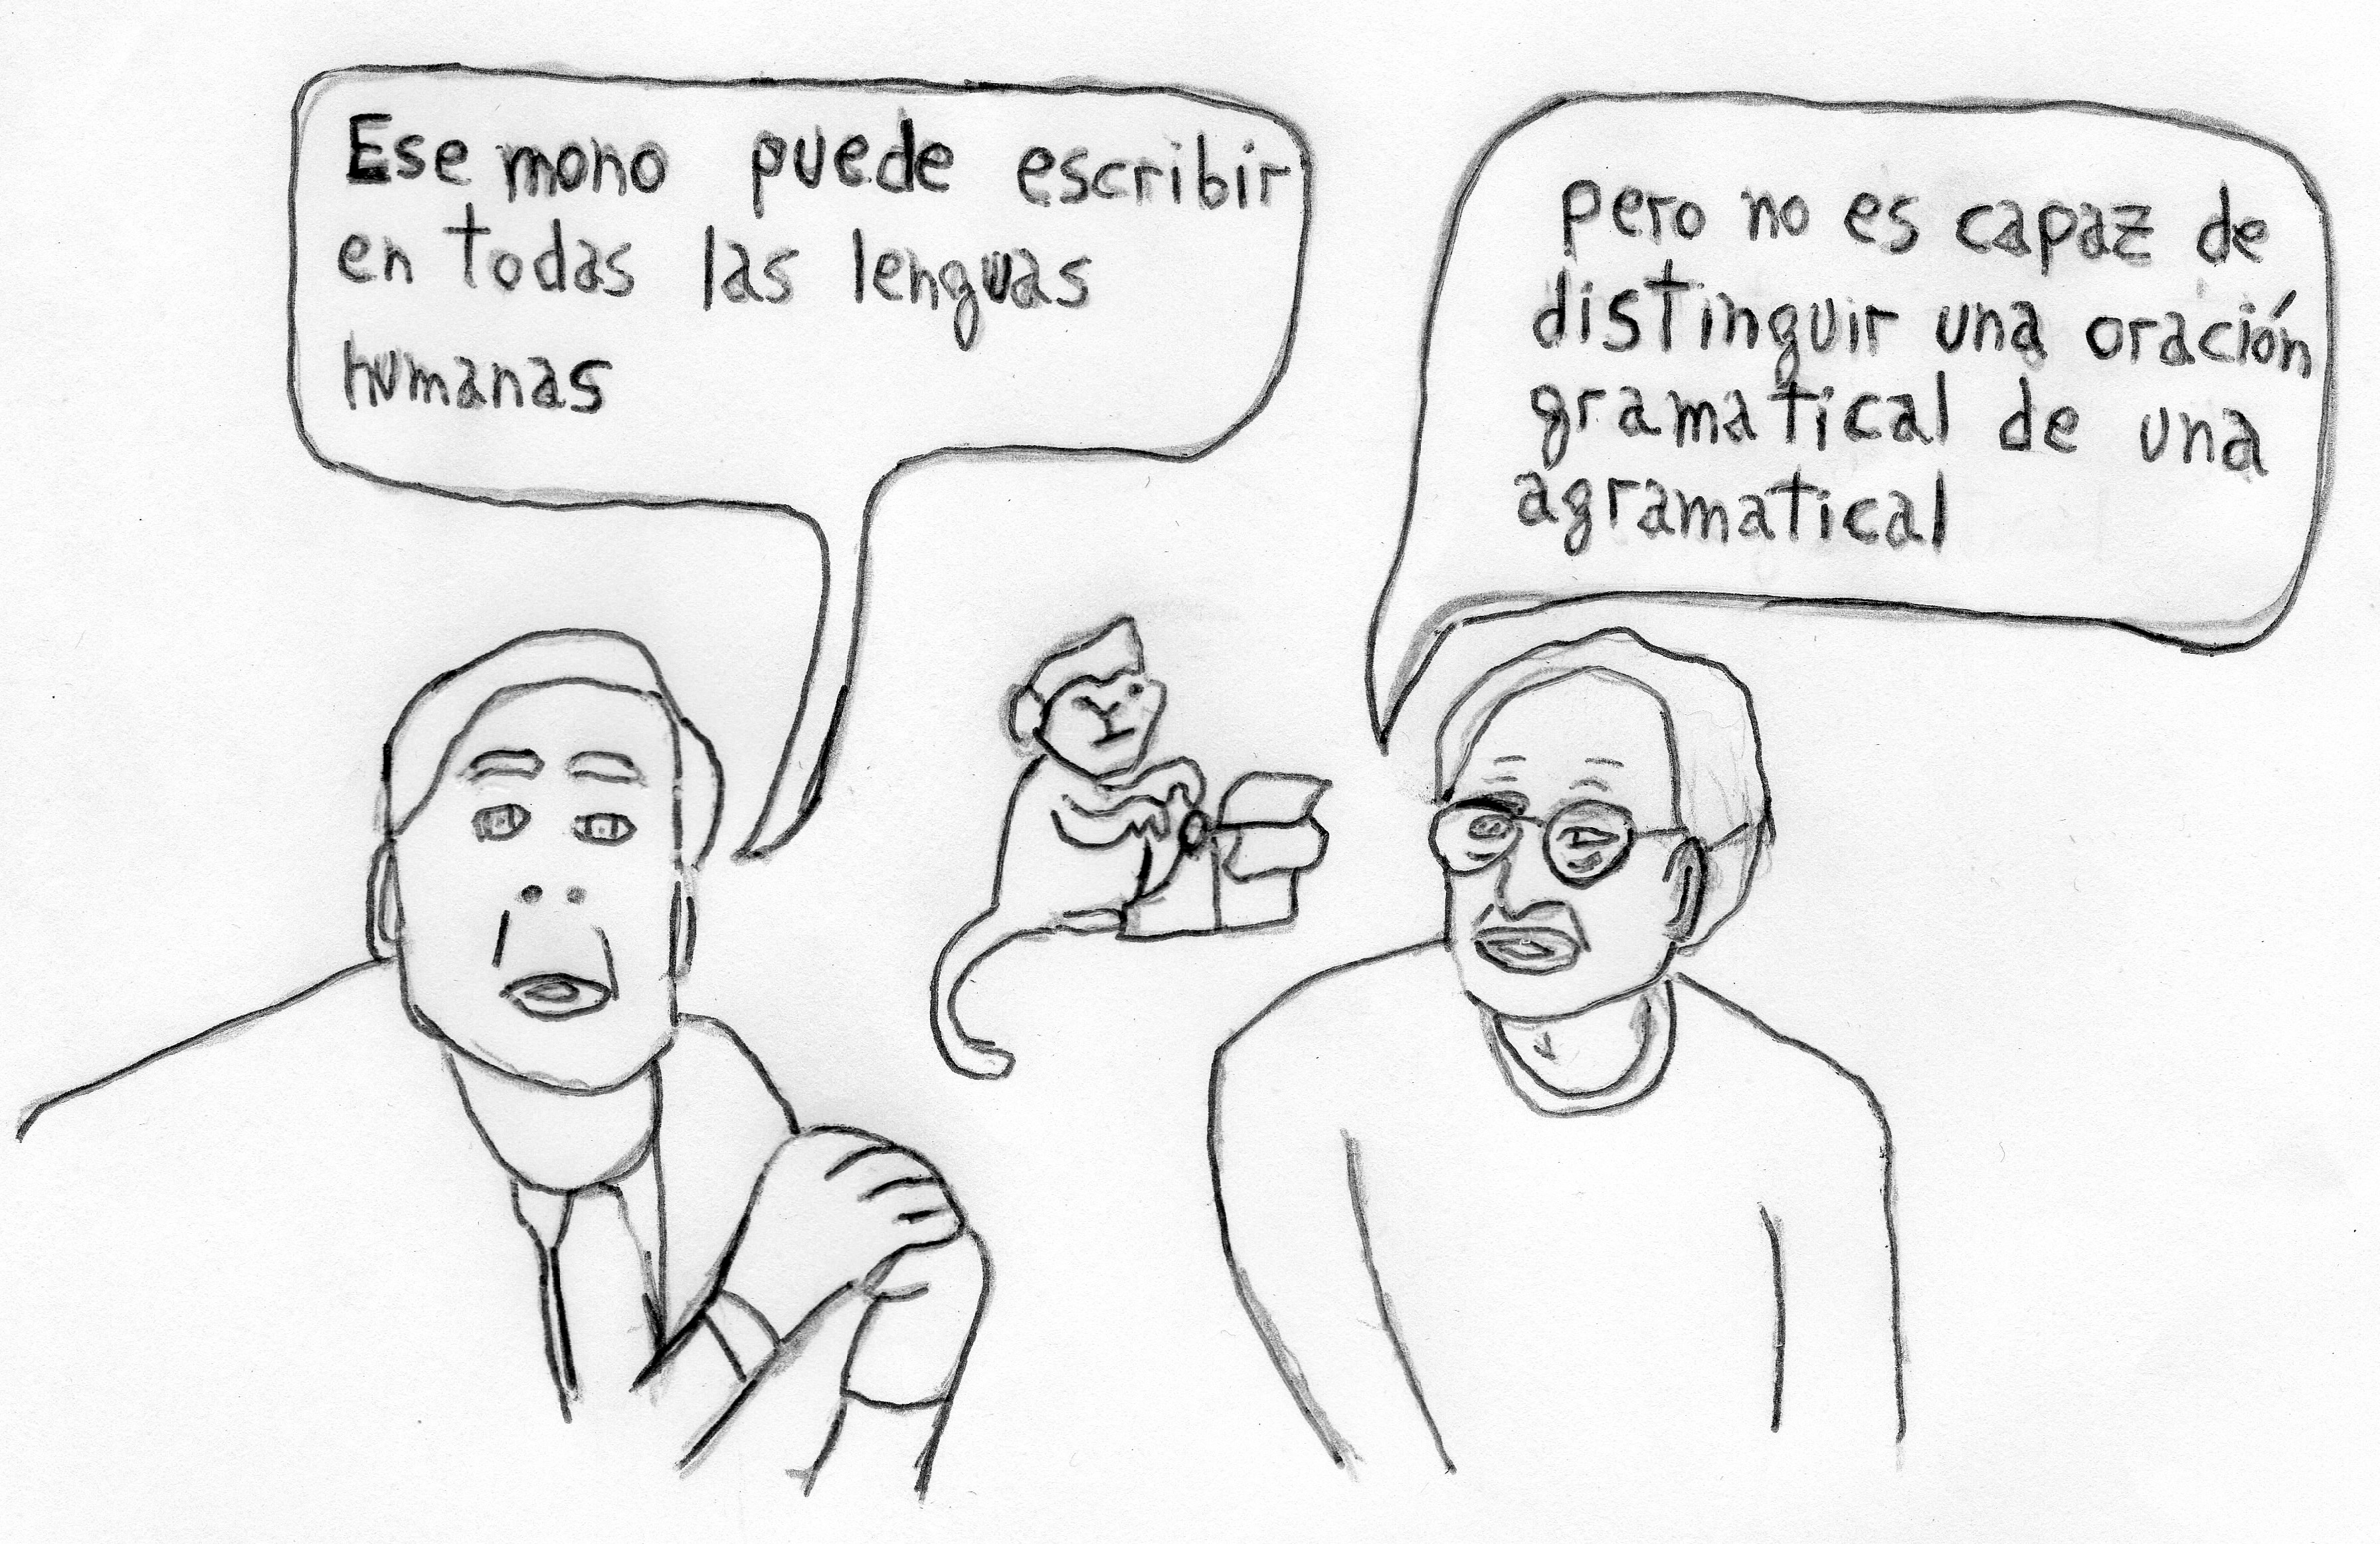
\includegraphics[width=\textwidth]{aux/mono.jpg}
\end{frame}

\section{Teoría de los lenguajes y lenguajes regulares}

\begin{frame}{Un poco de terminología}
\begin{itemize}
\item Denominamos \textit{alfabeto} al conjunto no vacío de símbolos discretos. En el caso de los textos digitales, estos serán caracteres pertenecientes a alguna fuente de codificación. El alfabeto se designa convencionalmente con la letra $\Sigma$
\pause
\item La concatenación de símbolos (iguales o diferentes) de un alfabeto $\Sigma$ se conoce con el nombre de cadena.
\end{itemize}
\end{frame}



\begin{frame}{$\Sigma$*}
$\Sigma$* equivale al conjunto de todas las cadenas posibles que se pueden obtener a partir de un alfabeto $\Sigma$.
\end{frame}

\begin{frame}{Lenguaje}

\begin{itemize}
\item Denominamos lenguaje a un conjunto de cadenas que está incluido en $\Sigma$*.
\end{itemize}

\end{frame}

\begin{frame}
Definir un lenguaje por extensión consiste en nombrar uno a uno todos sus miembros. Esto, por supuesto, es un método de definición de conjuntos totalmente inviable para lenguajes formados por infinitos elementos. En su lugar, hay que recurrir a un tipo de definición intensional.
\end{frame}


\begin{frame}
\begin{itemize}
\item Todo problema (e.g., ¿cuáles cadenas pertenecen al español?, ¿cuáles son las obras de Shakespeare?, etc.) se puede representar en términos de un lenguaje (e.g. el conjunto de cadenas del español, el conjunto de las obras de Shakespeare, etc.) y viceversa.
\item Así como hay problemas de diversa complejidad, los respectivos lenguajes también se clasifican según su complejidad. 
\end{itemize}
\end{frame}

\begin{frame}
\begin{itemize}
\item Las expresiones regulares son un sistema de notación que permite caracterizar la familia de lenguajes más sencillos: los llamados lenguajes regulares. \pause
\item Esa sencillez formal acarrea también un bajo costo de procesamiento, lo que vuelve a las expresiones regulares muy eficientes computacionalmente. \pause
\item Las expresiones regulares no sirven, entonces, para caracterizar conjuntos de cadenas más complejos, como el conjunto de las oraciones gramaticales del español o el conjunto de operaciones aritméticas bien resueltas. Pero permiten identificar lenguajes más sencillos, como el conjunto de las cadenas de caracteres alfanuméricos separados por puntos, el conjunto de las cadenas que tienen el formato de direcciones de correo electrónico, etc. \pause
\item Aplicado como problema, una expresión regular nos permite identificar cadenas de determinada naturaleza en el marco de un corpus, como el que elaboró el mono.
\end{itemize}
\end{frame}

\section{Convenciones notacionales de las expresiones regulares}

\begin{frame}
Primeramente, cualquier secuencia de caracteres del alfabeto $\Sigma$ = ASCII, escapando aquellos caracteres que oficien de operadores, es una expresión regular r que matcheará con esa secuencia de caracteres. 

\begin{center}\begin{figure}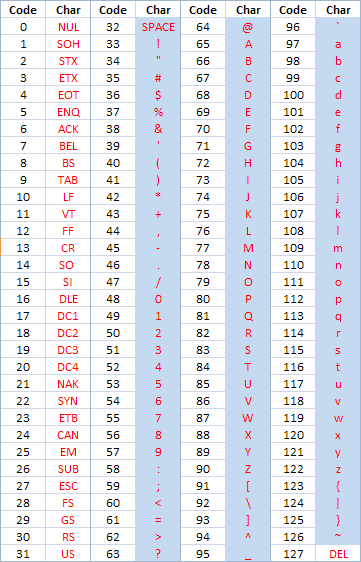
\includegraphics[width=0.35\textwidth]{aux/ascii-table.png}\caption{Tomado de \url{https://catonmat.net/my-favorite-regex}}\end{figure}\end{center}

\end{frame}

\begin{frame}
En la bibliografía teórica se utiliza la función interpretación $\llbracket\alpha\rrbracket$ para evaluar el significado de la expresión regular $\alpha$ (ver \citealt{Wintner:2010formallanguages}). 

Por ejemplo,
\begin{itemize}
\item $\llbracket$abc$\rrbracket$ = $\lbrace$w| w es una cadena formada por la concatenación de a, b y c$\rbrace$ = abc
\item $\llbracket$Fer$\rrbracket$ = $\lbrace$w| w es una cadena formada por la concatenación de F, e y r$\rbrace$ = Fer
\item y así sucesivamente.
\end{itemize}

\end{frame}

\begin{frame}{Paréntesis y estrella de Kleene}

\begin{itemize}
\item ()

Para delimitar bloques de cadenas

\item * 

cero o más ocurrencias del caracter o bloque anterior

Por ejemplo, $\llbracket$a*$\rrbracket$ = $\lbrace$w| w es una cadena formada por la concatenación de cero o más ocurrencias de a$\rbrace$

\begin{tabular}{|c|c|}\hline
$\llbracket$ab*$\rrbracket$ & {\begin{Form}\begin{tabular}{l}\TextField[width=0.70\textwidth, height=0.5cm, multiline=false]{}\\\\\end{tabular}\end{Form}}\\ \hline
$\llbracket$(ab)*$\rrbracket$ & {\begin{Form}\begin{tabular}{l}\TextField[width=0.70\textwidth, height=0.5cm, multiline=false]{}\\\\\end{tabular}\end{Form}}\\ \hline
\end{tabular}
\end{itemize}

\end{frame}

\begin{frame}{+ y ?}
\begin{itemize}
\item +

una o más ocurrencias del caracter o bloque anterior

Por ejemplo, $\llbracket$a+$\rrbracket$ = $\lbrace$w| w es una cadena formada por la concatenación de una o más ocurrencias de a$\rbrace$

\item ?

una o ninguna ocurrencia del caracter o bloque anterior

Por ejemplo, $\llbracket$ab?$\rrbracket$ = $\lbrace$a, ab$\rbrace$

\begin{tabular}{|c|c|}\hline
$\llbracket$ab+$\rrbracket$ & {\begin{Form}\begin{tabular}{l}\TextField[width=0.70\textwidth, height=0.5cm, multiline=false]{}\\\\\end{tabular}\end{Form}}\\ \hline
$\llbracket$(ab)+$\rrbracket$ & {\begin{Form}\begin{tabular}{l}\TextField[width=0.70\textwidth, height=0.5cm, multiline=false]{}\\\\\end{tabular}\end{Form}}\\ \hline
$\llbracket$(a?b)+$\rrbracket$ & {\begin{Form}\begin{tabular}{l}\TextField[width=0.70\textwidth, height=0.5cm, multiline=false]{}\\\\\end{tabular}\end{Form}}\\ \hline
\end{tabular}

\end{itemize}
\end{frame}

\begin{frame}

\begin{itemize}
\item {.}

cualquier caracter excepto cambio de línea

Por ejemplo, $\llbracket$a.$\rrbracket$ = $\lbrace$aa, ab, ac, ad...$\rbrace$)

\item $\lbrace$n$\rbrace$ 

n cantidad de ocurrencias del caracter o bloque anterior

Por ejemplo, $\llbracket$a$\lbrace$3$\rbrace\rrbracket$ = $\lbrace$aaa$\rbrace$)

\item $\lbrace$n,m$\rbrace$ 

entre n y m cantidad de ocurrencias del caracter o bloque anterior (cuando se usa para matchear, matchea con el menor número posible) 

Por ejemplo, $\llbracket$a$\lbrace$3,6$\rbrace\rrbracket$ = $\lbrace$aaa, aaaa, aaaaa, aaaaaa$\rbrace$)

\begin{tabular}{|c|c|}\hline
$\llbracket$Achi{$\lbrace$}2$\rbrace$s$\rrbracket$ & {\begin{Form}\begin{tabular}{l}\TextField[width=0.70\textwidth, height=0.5cm, multiline=false]{}\\\\\end{tabular}\end{Form}}\\ \hline
$\llbracket$(Bla)$\lbrace$3$\rbrace\rrbracket$ & {\begin{Form}\begin{tabular}{l}\TextField[width=0.70\textwidth, height=0.5cm, multiline=false]{}\\\\\end{tabular}\end{Form}}\\ \hline
$\llbracket$(Bla)$\lbrace$2,4$\rbrace\rrbracket$ & {\begin{Form}\begin{tabular}{l}\TextField[width=0.70\textwidth, height=0.5cm, multiline=false]{}\\\\\end{tabular}\end{Form}}\\ \hline
\end{tabular}

\end{itemize}

\end{frame}

\begin{frame}{Disyunción y rango}
\begin{itemize}
\item {} [] = disyunción entre lo que aparezca adentro ($\llbracket$[abcd]$\rrbracket$ = $\lbrace$a,b,c,d$\rbrace$)

\item {} [x-y] = rango de caracteres que aparecen entre x e siguiendo el orden de ASCII ($\llbracket$[a-d]$\rrbracket$ = $\lbrace$a,b,c,d$\rbrace$)

\item {} [$^{\wedge}$x] = expresiones que excluyan x.
\end{itemize}

El rango mayor que se puede obtener es [ -$\sim$]



\end{frame}

\begin{frame}{Abreviaturas}
\begin{itemize}
\item $\backslash$s = espacio en blanco
\item $\backslash$S = cualquier caracter que no sea un espacio en blanco
\item $\backslash$d = cualquier dígito.
\item $\backslash$D = cualquier símbolo que no sea un dígito
\item $\backslash$w = cualquier caracter alfanumérico
\end{itemize}


\end{frame}

\begin{frame}
Establecer las equivalencias en términos de rangos
\begin{tabular}{|c|c|c|}\hline
Abreviatura & rango \\ \hline
$\backslash$d & {\begin{Form}\begin{tabular}{l}\TextField[width=0.70\textwidth, height=0.5cm, multiline=false]{}\\\\\end{tabular}\end{Form}}\\ \hline
$\backslash$w &  {\begin{Form}\begin{tabular}{l}\TextField[width=0.70\textwidth, height=0.5cm, multiline=false]{}\\\\\end{tabular}\end{Form}}\\ \hline
\end{tabular}

\end{frame}


\begin{frame}

\begin{tabular}{|c|c|c|}\hline
Expresiones target & Expresión regular \\ \hline 
Edad (en arábigos) & {\begin{Form}\begin{tabular}{l}\TextField[width=0.40\textwidth, height=0.5cm, multiline=false]{}\\\\\end{tabular}\end{Form}}\\ \hline
Estructura de sílaba & {\begin{Form}\begin{tabular}{l}\TextField[width=0.40\textwidth, height=0.5cm, multiline=false]{}\\\\\end{tabular}\end{Form}}\\ \hline
Perífrasis terminativas &  {\begin{Form}\begin{tabular}{l}\TextField[width=0.40\textwidth, height=0.5cm, multiline=false]{}\\\\\end{tabular}\end{Form}}\\ \hline
\end{tabular}


\end{frame}

\begin{frame}
Páginas para probar expresiones regulares: 

\begin{itemize}
\item \url{https://regex101.com/}
\item \url{https://regexr.com/}
\end{itemize}

\end{frame}

\begin{frame}[allowframebreaks]{Bibliografía}
\nocite{HopcroftMotwaniUllman:2006automata}
\nocite{jurafskyspeech}
\bibliography{aux/biblio}
\bibliographystyle{aux/apalike-es}
\end{frame}

\end{document}